\documentclass[crop,border={2pt 2pt 2pt 2pt},tikz]{standalone}
\usepackage{braket}
\usepackage{bbold}
\usepackage{bm}
\usepackage{amsmath}

\usetikzlibrary{backgrounds,decorations.markings, calc}
\tikzset{>=latex}
\tikzset{->-/.style={decoration={
  markings,
  mark=at position .55 with {\arrow{>}}},postaction={decorate}}}
\begin{document}
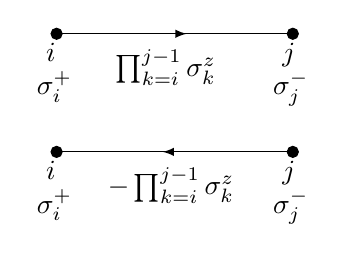
\begin{tikzpicture}

    \coordinate[draw] (i) at (0,0);
    \coordinate[draw] (j) at (3,0);

    \draw[fill, black] (i) circle (2pt);
    \draw[fill, black] (j) circle (2pt); 



    \node[text width = 0.5cm, anchor= north] at (i) {$\ i $ \\ $\sigma_i ^{+}$};
    \node[text width = 0.5cm, anchor= north] at (j) {$\ j $ \\ $\sigma_j ^{-}$};

    \draw[->-, black] (i) -- (j);

    \node[text width = 1.5cm, anchor= north] at ($(i) + 0.5*(j)$) {   \\  $ \prod_{k=i}^{j-1} \sigma_k ^{z}$};


    \begin{scope}[yshift = -1.5cm]
        \coordinate[draw] (i) at (0,0);
        \coordinate[draw] (j) at (3,0);
        \draw[fill, black] (i) circle (2pt);
        \draw[fill, black] (j) circle (2pt); 


        \node[text width = 0.5cm, anchor= north] at (i) {$\ i $ \\ $\sigma_i ^{+}$};
        \node[text width = 0.5cm, anchor= north] at (j) {$\ j $ \\ $\sigma_j ^{-}$};

        \draw[->-, black] (j) -- (i);

        \node[text width = 1.7cm, anchor= north] at ($(i) + 0.5*(j)$) {   \\  $ -\prod_{k=i}^{j-1} \sigma_k ^{z}$};

    \end{scope}

    

\end{tikzpicture}
\end{document}
 
